%============================================================
%     Group Meeting Report Template — Computational Imaging
%============================================================
\documentclass[15pt]{beamer}
\makeatletter
\makeatother

%======================== packages & settings ========================
\usepackage{amsmath, pifont, bookmark, tabularx, booktabs, adjustbox, graphicx, caption, subcaption, listings, color, tikz}
\usetikzlibrary{arrows.meta,positioning,shapes.geometric,shapes.misc,fit,calc,decorations.pathreplacing}
\usepackage{hyperref}
\hypersetup{colorlinks=true,linkcolor=blue,urlcolor=blue}

%======================== theme & fonts ========================
\usetheme{Montpellier}
\renewcommand{\familydefault}{\sfdefault}

% TOC numbered
\setbeamertemplate{section in toc}[sections numbered]
\setbeamertemplate{subsection in toc}[subsections numbered]

% footer
\setbeamerfont{footline}{size=\tiny}
\setbeamertemplate{footline}{
  \leavevmode
  \hfill \insertframenumber{} / \inserttotalframenumber \hspace{2ex}\vskip2pt}

% title fonts
\setbeamerfont{title}{size=\fontsize{20pt}{24pt}\selectfont}
\setbeamerfont{subtitle}{size=\fontsize{12pt}{14.4pt}\selectfont}
\setbeamerfont{author}{size=\fontsize{10pt}{12pt}\selectfont}
\setbeamerfont{date}{size=\fontsize{10pt}{12pt}\selectfont}

%======================== macros ========================
\newcommand{\Obj}{\mathrm{O}}
\newcommand{\Probe}{\mathrm{P}}
\newcommand{\Exit}{\psi}
\newcommand{\uu}{\mathbf{u}}
\newcommand{\rr}{\mathbf{r}}
\newcommand{\Rj}{\mathbf{R}_j}
\newcommand{\kk}{\mathbf{k}}

\tikzset{
  >=Stealth,
  line/.style      = {->, thick},
  block/.style     = {rectangle, rounded corners, draw, align=left, thick, inner sep=6pt, fill=white},
  io/.style        = {trapezium, trapezium left angle=70, trapezium right angle=110, draw, thick, align=left, inner sep=6pt, fill=white},
  smallblock/.style= {rectangle, rounded corners, draw, align=left, thick, inner sep=4pt, fill=white, font=\small},
  loopbox/.style   = {rectangle, rounded corners, draw, dashed, thick, inner sep=8pt},
  note/.style      = {rectangle, draw, align=left, inner sep=4pt, fill=white, font=\scriptsize}
}

%======================== basic info ========================
\title{Weekly Research Report}
\subtitle{}
\author{Zihan Xu}
\date{\today}

%============================================================
\begin{document}

%---------------- title ----------------
\begin{frame}[plain]
  \titlepage
\end{frame}
\addtocounter{framenumber}{-1}

%---------------- toc ----------------
\begin{frame}[plain]{Outline}
  \tableofcontents[sectionstyle=show, subsectionstyle=hide]
\end{frame}
\addtocounter{framenumber}{-1}

%============================================================
\section{Weekly Progress Overview}
%============================================================
\begin{frame}{Summary of This Week}

\begin{itemize}
  \item Read three key papers for theoretical and algorithmic understanding:
  \begin{itemize}
    \item \textit{High-Resolution Scanning X-ray Diffraction Microscopy}
    \item \textit{Further Improvements to the Ptychographical Iterative Engine}
    \item \textit{X-ray Ptychography with Highly-Curved Wavefront}
  \end{itemize}

  \item Implemented and tested the \textbf{mPIE (momentum-based PIE)} algorithm in Python.

  \item Established a new \textbf{lab Git repository} for shared code management and collaboration.
\end{itemize}

\end{frame}


%============================================================
\section{Probe Complexity and Reconstruction Quality}
%============================================================
\begin{frame}{Effect of Probe Complexity on Reconstruction}
%------------------------------------------------------------

\begin{columns}[T,onlytextwidth]
% ---------- LEFT COLUMN ----------
\begin{column}{0.55\textwidth}

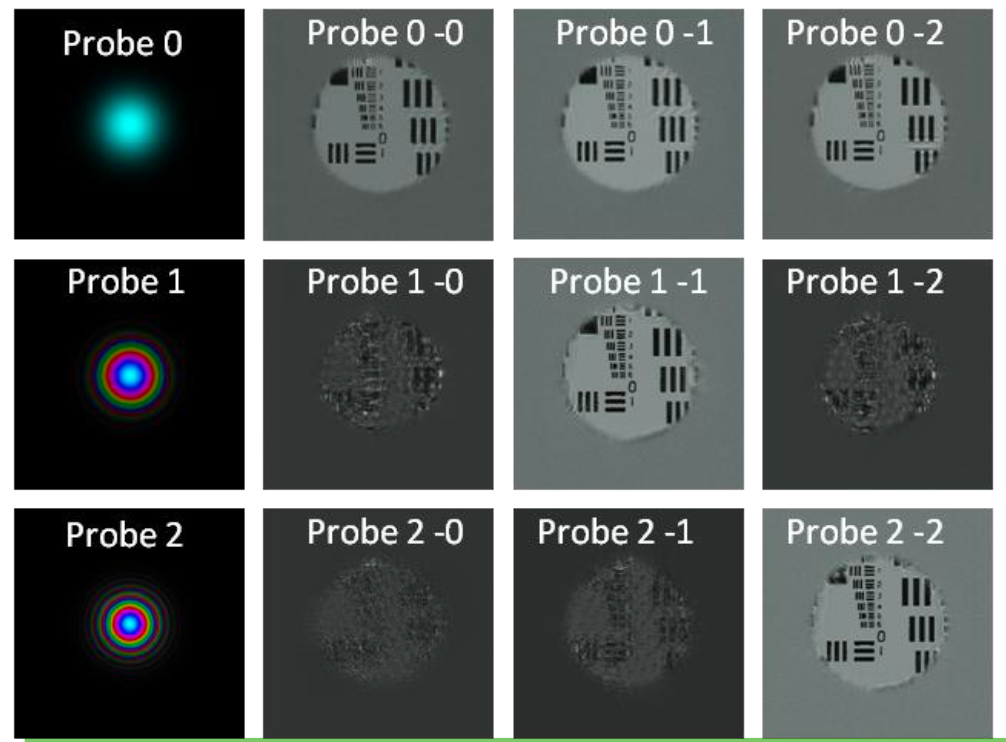
\includegraphics[width=0.7\linewidth]{Probes.png}
\end{column}

% ---------- RIGHT COLUMN ----------
\begin{column}{0.45\textwidth}
\centering

\includegraphics[width=\linewidth]{figure2.png}


\end{column}
\end{columns}
A complex, physically realistic probe (with curvature or structure) gives richer information and better reconstructions — but only if the algorithm can model or learn it accurately; otherwise, the same complexity causes convergence instability.
\end{frame}



%============================================================
\section{Experimental / Simulation Results}
%============================================================
\begin{frame}{Simulation Results}

    \centering
    \includegraphics[width=\linewidth]{figure3.png}
    the curved probe performs better than the flat or pinhole like probe, and the more complex the probe is , the better the outcome of reconstruction is. But more complex probe also lead to guess accuracy problem.
\end{frame}



%============================================================
\section{mPIE Simulation}
%============================================================
\begin{frame}{mPIE simulation}
    \centering
    \includegraphics[width=0.5\linewidth]{figure4.png}
   
\textbf{mPIE Update (with Momentum):}
\[
O_{n+1} = O_n +
\beta \frac{|P|}{P_{\max}}
\frac{P^{*}}{|P|^2+\alpha}
\big(\Psi_{c,n}-\Psi_{g,n}\big)
+ \gamma (O_n - O_{n-1})
\]
\end{frame}

\begin{frame}{Comparison of the SSE of PIE family}
    \centering
    \includegraphics[width=0.5\linewidth]{figure5.png}
   \\ mPIE with adaptive beta shows better convergence performance than standard PIE and fixed-beta mPIE, especially in the later stage of iteration.
\end{frame}

%============================================================
\section{Future Plan}
%============================================================
\begin{frame}{Plans for Next Week}
\footnotesize
\begin{itemize}
  \item [\ding{43}] Finish reading mPIE relevant papers.
  \item [\ding{43}] Read related works on Ptychography noise reduction and robustness.
  \item [\ding{43}] Reorganize my codes and pack my code into functions.
\end{itemize}
\end{frame}

%============================================================
\section*{Acknowledgement}
%============================================================
\begin{frame}[plain]
\centering
\vspace{1cm}
\Huge Thank You!\\[3mm]
\large Questions and Discussion
\end{frame}

\end{document}
